\documentclass[11pt]{article}
\usepackage[margin=1.5cm]{geometry}
\usepackage{graphicx}
\usepackage{amsmath}
\usepackage{float}
\usepackage{wrapfig}
%\usepackage[compact]{titlesec}  
%\titlespacing{\section}{0pt}{0pt}{0pt}
%\titlespacing{\subsection}{0pt}{0pt}{0pt}


\begin{document}
\begin{center}
    IVR Assignment

    B156771 \& B163370
\end{center}
%\maketitle
\section{Vision}
\subsection{Estimating Joint Angles}
\subsubsection{Methodology}
The algorithm employed makes use of the two orthogonal projections provided by the cameras to provide a 3D point/vector for each joint, and therefore requires both \texttt{image1.py}, and \texttt{image2.py} to be run simultaneously.
The two cameras estimate the point of the joint in their respective projection using the joints colour and a blob-detection approach.
In the event that a joint is hidden from one of the camera, its previous position is sent on the stream instead.
Furthermore, the estimated points are transformed so that the origin is given by joint 1 -- the yellow joint at the base -- and then translated to metres from pixel coordinates. 
These estimates along with the plane it represents are sent to a third program (\texttt{consume\_images.py}), which reads the points off these streams and combines them using the value for the $z$ position, which is the common axis. 
Care had to be taken due to the multiple streams and asynchronous nature of the processing. 
For this, a thread lock was used to minimise the possibility of race conditions affecting the readings. 
With the joint positions collected and merged effectively, the angle is calculated using the definition of the dot product of vectors.
I.e., given two joint's positions $\vec{j_1}$ and $\vec{j_2}$, where the vector given by the link between them is given by $\vec{l_{1,2}} = \vec{j_2} - \vec{j_1}$; its angle with respect to $\vec{u_k}$, the unit vector along the $k$ axis, is given by $$ \theta = \arccos\left(\frac{\vec{l_{1,2}}\cdot \vec{u_k}}{||\vec{l_{1,2}}||}\right) - \frac{\pi}{2}.$$
The angle is shifted by a factor of $\pi/2$ to account for the range of motion of the joints.
The results of this process is given below (estimates are in blue, actual angles are in red):

\begin{figure}[!htb]
\minipage{0.32\textwidth}
    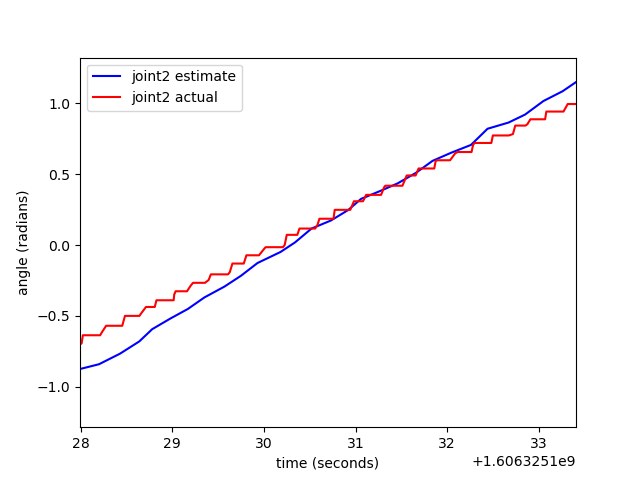
\includegraphics[width=\linewidth]{../figures/joint2.png}
    \caption{Joint 2 estimates vs actual position}
\endminipage\hfill
\minipage{0.32\textwidth}
    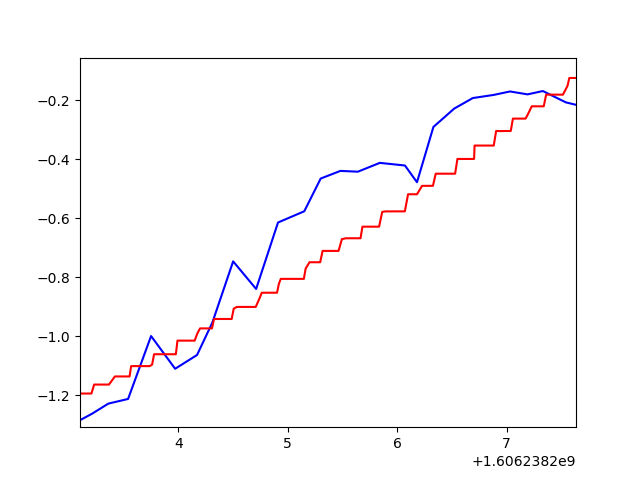
\includegraphics[width=\linewidth]{../figures/joint3.png}
    \caption{Joint 3 estimates vs actual position}
\endminipage\hfill
\minipage{0.32\textwidth}
    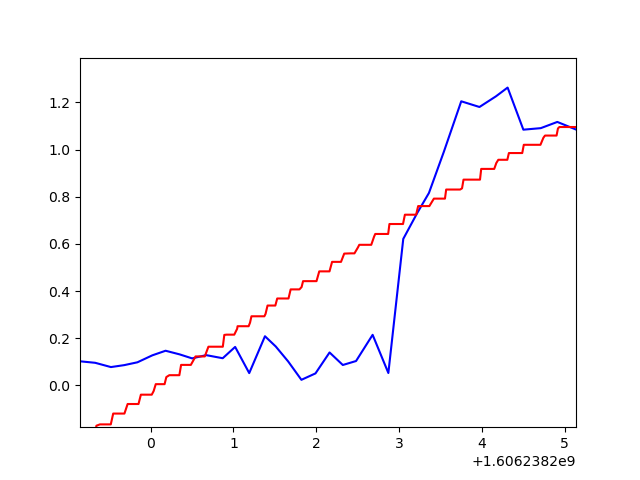
\includegraphics[width=\linewidth]{../figures/joint4.png}
    \caption{Joint 4 estimates vs actual position}
\endminipage\hfill
\end{figure}

\subsubsection{Potential Improvements}
From the figures above, it is clear that the estimate of the fourth joint leaves much to be desired.
We would hypothesise that the primary source of error for this joint's estimated angle would be the handling of the joint being out of sight of the camera.
Given its positioning on the robot, it would be the most likely out of the four joints to be hidden from view at any given point.
Perhaps instead of assuming the previous position of the joint when it disappears from view, we could instead perform a linear interpolation between the last recorded position, and the next recorded position -- effectively taking the average between the two.
Taking this a step even further, we could potentially use a more advanced interpolation technique and estimate the trajectory while taking position measurements, substituting these approximations when an actual value cannot be determined.
While this would lead to potentially smaller errors, we would need to consider the requirements of the application.
Should speed of processing be more important, the method employed would be more suitable as the number of operations to perform per measurement would be minimal.
If, instead, accuracy were more critical, then this method may prove to be more fruitful despite being more computationally expensive. 

\subsection{Target Detection}
For this task we extended the work done in the previous part. 
We isolate the two potential objects using the orange colour range and blob detection. 
From there, we use a template of the orange sphere taken from one of the cameras to isolate the sphere's position. 
The centroid of the two potential matches are taken, and then a cropped sample of each retrieved from the frame. 
From there, each sample is compared with the template. 
The sample with the smaller distance is assumed to be the sphere, and its coordinates, along with a time stamp is returned.
After normalizing the position with respect to joint 1 or the base of the robot, the positions estimated from each camera is sent on the stream \texttt{target\_est} which is read from third script, \texttt{track\_target.py}. 
Much like in the previous part, the two coordinates are joined along the $z$ position where the difference in time stamp is used to determine whether or not two points from each camera correspond to the same reading. 
In this case as well as in the above part, a difference of less than 10 milliseconds is needed for two readings to be considered separate parts of the same point.  
For the $z$ position, the former of the two readings is used; and a thread lock prevents any potential race conditions. 
Lastly, the actual positions are read from their respective streams: \texttt{target/x\_position\_controller/command}, and its counterparts.
We note that the script \texttt{target\_move.py} was not used.
This script caused the target to move erratically leading to illegible plots as well as inaccurate readings.
Since the target and its decoy were already following a sinusoidal movement around the robot, it was decided that the script was not needed. 
Below we plot the estimated positions per dimension along with the actual reading as given by their respective streams.
\begin{figure}[!htb]
\minipage{0.32\textwidth}
    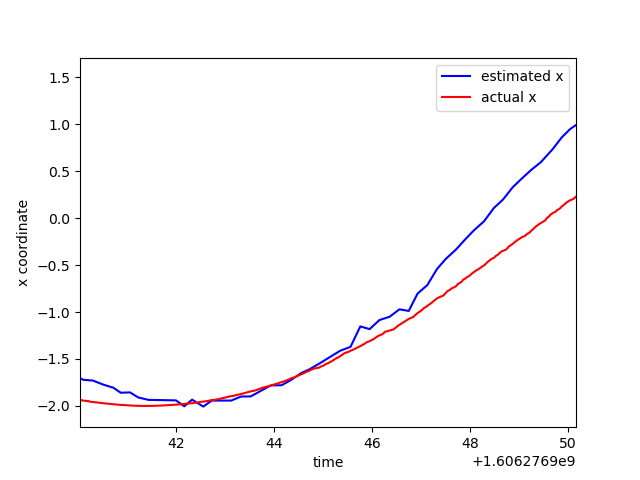
\includegraphics[width=\linewidth]{../figures/est_x_pos.png}
    \caption{Estimated $x$ coordinate}
\endminipage\hfill
\minipage{0.32\textwidth}
    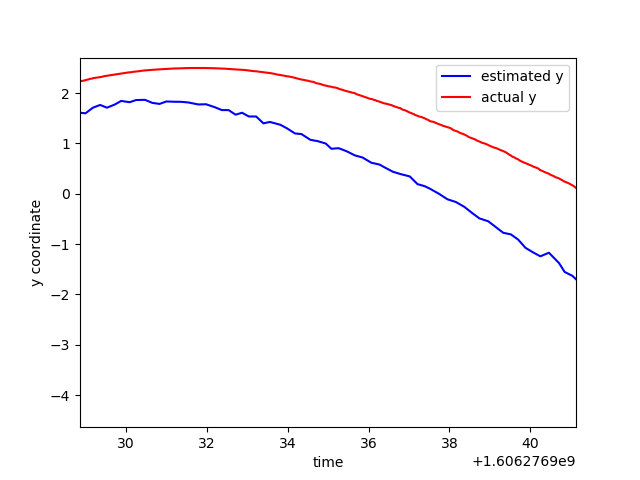
\includegraphics[width=\linewidth]{../figures/est_y_pos.png}
    \caption{Estimated $y$ coordinate}
\endminipage\hfill
\minipage{0.32\textwidth}
    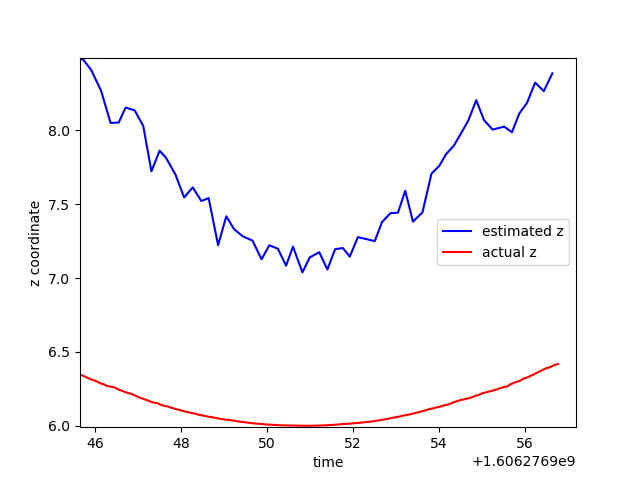
\includegraphics[width=\linewidth]{../figures/est_z_pos.png}
    \caption{Estimated $z$ coordinate}
\endminipage\hfill
\end{figure}
We can see that the readings for the $x$ and $y$ estimates seem to be decently accurate, with an error of less than a metre.
The $z$ estimate; however, is once again difficult. 
Having an average error of about three metres, this reading is clearly too inaccurate. 
Nevertheless, the path that the estimate takes is similar if not equal to that of the actual readings, meaning that the majority of the error is likely caused by a miscalculation in either the normalization of the position or the conversion from pixel to metres. 
Given that the other estimates seem to line up fairly decently, we would expect that the error would lie in the normalization process. 

\section{Joint 1 Movements}

The algorithm here will follow very similarly to that detailed in section 1. 
The difference here will be in determining the angle of joint 1 as it is along the $z$ axis, and so the same method will not be as fruitful.
The key observation here is that if we look at the robot top-down, we notice that the link between joints 2/3 and 4 show the angle by which joint 1 is rotated. 
The important assumption is that joint 1 is precisely at the origin; however, we insured this was the case as explained in section 1. 
We used the data as it was collected in section 1, and this time took the $x,y$ coordinates of joint 4 and passed it into the $\arctan2$ function.
We then used the same method as above in determining the angles for the remaining joints. 
This process yielded the following plots:

\begin{figure}[!htb]
\minipage{0.45\textwidth}
    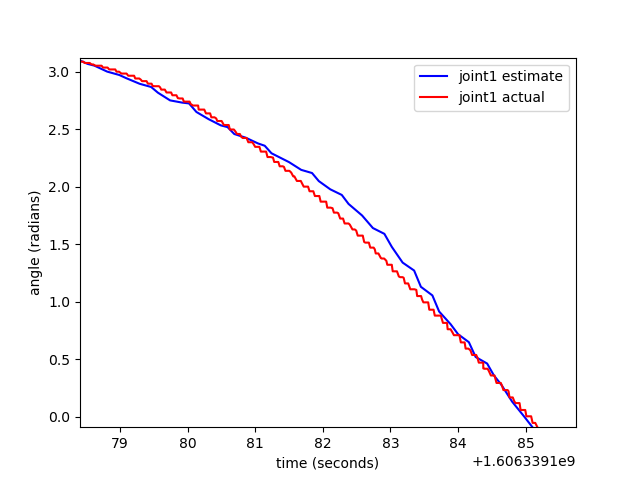
\includegraphics[width=\linewidth]{../figures/joint1.png}
    \caption{Estimated joint 1 angle}
\endminipage\hfill
\minipage{0.45\textwidth}
    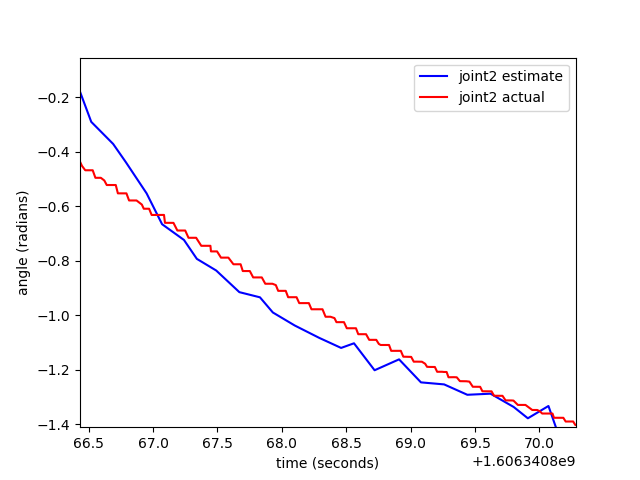
\includegraphics[width=\linewidth]{../figures/04_joint2.png}
    \caption{Estimated joint 2 angle}
\endminipage\hfill
\minipage{0.45\textwidth}
    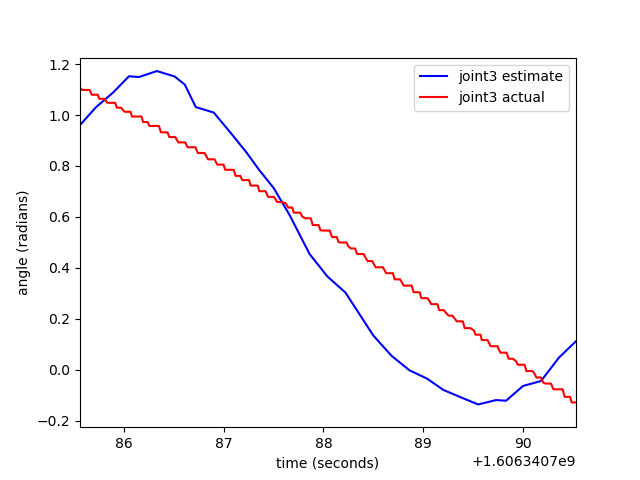
\includegraphics[width=\linewidth]{../figures/04_joint3.png}
    \caption{Estimated joint 3 angle}
\endminipage\hfill
\minipage{0.45\textwidth}
    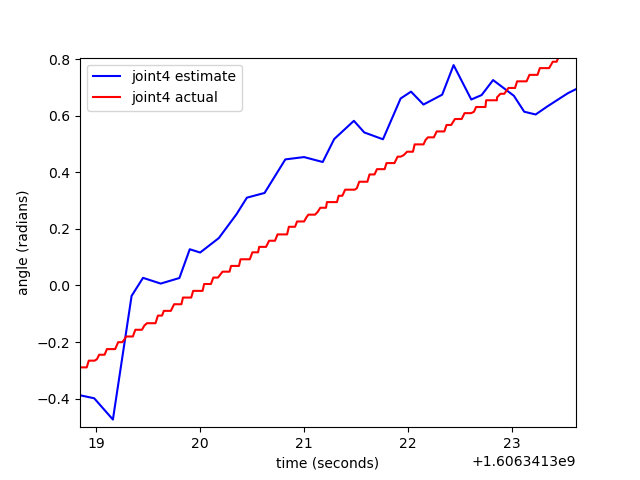
\includegraphics[width=\linewidth]{../figures/04_joint4.png}
    \caption{Estimated joint 4 angle}
\endminipage\hfill
\end{figure}

The results we found for joint 1 were exactly as we had hoped. 
The remaining joints, while some suffered larger errors, were able to retain sufficient accuracy for short periods of time. 
In the case of joint 4, compared to the plot in section 1, we would argue that it is now more accurate than before, which is an unexpected, but not unwelcomed result. 
We should note; however, that for extended periods of observation, errors around the local maximum and minimum were much more pronounced.
This is certainly due to the increased degree of freedom in the robots movements, as well as the inherent loss of information given by the projection from 3 to 2 dimensions. 
While the angle between the joints may be moving as determined by their respective sinusoidal functions, because multiple joints are moving freely, when projected onto two dimension, the angle would give the appearance of either not changing at all, or changing only slightly. 
This would result in the more flattened areas near the local extremes. 
Furthermore, by rotating around the $z$ axis, the changes in the angle may not always be visible, depending on the degree to which joint 1 is rotated. 
These two facts combines make it significantly more challenging to accurately determine the angle of the joints.

\section{Robot Control}
\subsection{Forward Kinematics}

The robot in question is of type 4R spatial. Following are the DH parameters. The robot at its home position had few initial values.

\begin{table}[h]
\centering
\begin{tabular}{|l|l|l|l|l|l|}
Link \# & Aplha       & a   & d   & Theta    & Initial Joint Values \\\hline
1       & 90 degrees  & 0.0 & 2.5 & Variable & 90 degrees           \\\hline
2       & 90 degrees  & 0.0 & 0.0 & Variable & 90 degrees           \\\hline
3       & -90 degrees & 3.5 & 0.0 & Variable & 0 degree             \\\hline
4       & 0.0         & 3.0 & 0.0 & Variable & 0 degree             \\\hline    
\end{tabular}
\caption{DH parameters of the 4R spatial robot}
\end{table}

The translation co-ordinates from the homogeneous transformation matrix (HTM) of the robot are derived as below.

\[
\begin{bmatrix}
    e_{x}       & \\
    e_{y}       & \\
    e_{z}       &
\end{bmatrix}
=
\begin{bmatrix}
c1c2c3c4l4+s1s3c4l4-c1s2s4l4+c1c2c3l3+s1s3l3 & \\
s1c2c3c4l4-c1s3c4l4-s1s2s4l4+s1c2c3l3-c1s3l3 & \\
s2c3c4l4+c2s4l4+s2c3l3+l1
\end{bmatrix}
\]

At its home position when all the variable angles are 0.0 Radian the coordinates are derived as [0.0,0.0,9.0] which is correct as the end-effector is 9.0 units away along the Z axis.

\begin{table}[h]
\centering
\begin{tabular}{|l|l|l|l|l|l|}
X\_htm & Y\_htm & Z\_htm & X\_cv & Y\_cv & Z\_cv  \\\hline
5.44   & 1.63   & 1.87   & -0.62 & 5.69  & 5.56   \\\hline
4.29   & 0.74   & 1      & -1.3  & 4.86  & 6.46   \\\hline
3.91   & 3.57   & 0.38   & 0.28  & 6.2   & 3.3    \\\hline
4.66   & 2.13   & -0.02  & 0.11  & 5.94  & 4.86   \\\hline
3.69   & 4.31   & 1.87   & 0.44  & 5.82  & 2.53   \\\hline
5.67   & 1.98   & 2.36   & 0.02  & 5.81  & 5.13   \\\hline
5.67   & 0.66   & 2.33   & -1.04 & 5.51  & 5.77   \\\hline
5.48   & 1.6    & 2.67   & -0.5  & 5.48  & 5.95   \\\hline
5.66   & 0.44   & 1.87   & -1.46 & 5.49  & 5.6    \\\hline
2.77   & 4.31   & -0.02  & 0.42  & 5.96  & 2.4    \\\hline
\end{tabular}
\caption{Comparison of the joint angles calculated by HTM and CV}
\end{table}

We observed discrepancies between the coordinates coming from two different calculations.

\subsection{Closed-loop control}

We derived the Jacobian of the robot from the translation co-ordinates calculated from the previous section. The error is calculated as the difference between the desired end-effector position (which in our case is the position of the Orange spherical object) and the current end-effector position. We tuned the P-Gain and D-Gain parameters to make the robot trajectory smoother as much as we could.

Following are the different components of the derived Jacobian.

\
Effect of \textbf{joint1} velocity on end-effector velocity
=
\begin{bmatrix}
-s1c2c3c4l4+c1s3c4l4+s1s2s4l4-s1c2c3l3+c1s3l3 & \\
c1c2c3c4l4+s1s3c4l4-c1s2s4l4+c1c2c3l3+s1s3l3 & \\
0.0
\end{bmatrix}
\

\
Effect of \textbf{joint2} velocity on end-effector velocity
=
\begin{bmatrix}
-c1s2c3c4l4-c1c2s4l4-c1s2c3l3 & \\
-s1s2c3c4l4-s1c2s4l4-s1s2c3l3 & \\
c2c3c4l4-s2s4l4+c2c3l3
\end{bmatrix}
\

\
Effect of \textbf{joint3} velocity on end-effector velocity
=
\begin{bmatrix}
-c1c2s3c4l4+s1c3c4l4-c1c2s3l3+s1c3l3 & \\
-s1c2s3c4l4-c1c3c4l4-s1c2s3l3-c1c3l3 & \\
-s2s3c4l4-s2s3l3
\end{bmatrix}
\

\
Effect of \textbf{joint4} velocity on end-effector velocity
=
\begin{bmatrix}
-c1c2c3s4l4-s1s3s4l4-c1s2c4l4 & \\
-s1c2c3s4l4+c1s3s4l4-s1s2c4l4 & \\
-s2c3s4l4+c2c4l4
\end{bmatrix}
\

Here is some text that will hopefully wrap around the figure! 

Lorem ipsum dolor sit amet, consectetur adipiscing elit. Phasellus nibh sapien, finibus a nibh sit amet, finibus fringilla leo. Cras quam dui, pellentesque posuere turpis eget, accumsan commodo purus. Ut egestas nunc in est hendrerit, vel tincidunt justo semper. Praesent finibus suscipit viverra. Nam dui sem, dapibus aliquet dolor et, dignissim imperdiet diam. Sed sed metus porttitor, lobortis neque eget, posuere mauris. Suspendisse ornare lacus eu ligula congue cursus.
\begin{wrapfigure}{l}{0.2\textwidth}
\begin{center}
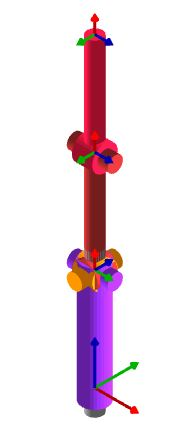
\includegraphics[scale=0.5]{report/3d_frame.JPG}
\caption{Frame Assignment Diagram}
\end{center}
\end{wrapfigure}
Aenean eu sem congue, pellentesque ex sed, imperdiet magna. Nam a tristique sem. Praesent id accumsan ante. Donec tempor consectetur erat, porta malesuada massa blandit eu. Proin id vulputate elit. Donec quis arcu sit amet sapien vehicula blandit. Interdum et malesuada fames ac ante ipsum primis in faucibus. Fusce sapien enim, tempor a dapibus ut, porttitor et justo.

Cras faucibus eleifend nulla, a vehicula ante fringilla sagittis. Quisque semper elit id est scelerisque, sollicitudin pretium est mattis. Morbi ultricies in elit nec vehicula. Morbi in magna vitae nulla egestas laoreet non sed ex. Quisque viverra eros nec nisl auctor, eu ultrices sapien vestibulum. Vestibulum et dolor malesuada, pharetra mi et, condimentum turpis. Morbi consequat volutpat facilisis. Aliquam justo augue, condimentum in tristique a, pulvinar vel purus. Quisque vestibulum odio non dui aliquet accumsan. Cras placerat bibendum nulla, ac tempor leo malesuada non. Etiam at mattis nulla.

Morbi nec pretium lorem. Nulla hendrerit feugiat augue eu congue. Duis et diam in sapien volutpat egestas. Duis et nisl sit amet nulla bibendum vestibulum. Aliquam laoreet interdum lectus. Nam at ornare libero. Vivamus congue mollis eros sit amet faucibus. Suspendisse mollis orci at urna fermentum, volutpat mattis dui ornare. Sed sit amet libero est. Nam sollicitudin sapien at feugiat hendrerit. Pellentesque eu quam ligula. Maecenas pulvinar elit nunc, quis tempor lacus tincidunt nec. Duis ornare ornare elit, nec ullamcorper mi iaculis eu. Fusce venenatis sit amet erat ut aliquam. Mauris fringilla, neque nec sagittis faucibus, mauris augue mattis metus, sed sagittis ipsum orci vel metus. Quisque ac pulvinar justo.

Cras lobortis elit ac blandit vulputate. Vestibulum ante ipsum primis in faucibus orci luctus et ultrices posuere cubilia curae; Morbi sit amet laoreet leo. Quisque dapibus augue in purus elementum scelerisque. Nam semper dui eu orci consequat tempor. Morbi lacus quam, fringilla sit amet suscipit quis, posuere vitae elit. Vestibulum eros orci, rhoncus nec imperdiet eu, aliquet vitae elit. Fusce aliquam tincidunt orci id posuere. 


\end{document}
